\mysubsection{Sarah Häfele}{Call to Action}\label{ssec:CtA}

Die Vermutung, dass bei einer Installation mit Musik und der Notwendigkeit, sich zu bewegen, die Hemmschwelle diese zu nutzen höher liegt, liegt nahe. Neben Lichteffekten durch die Scheinwerfer und dem offiziellen Spielfeld dienen deswegen weitere Komponenten zur \textit{Call to Action}, also zur Motivation der Besucher. Diese sollen nicht nur zum Mitmachen bewegen, sondern auch gleichzeitig anleitend wirken.

\subsubsection{Der Presentation-Screen}

Der Presentation-Screen ist als eine Art Präsentationsfläche gedacht, die den Nutzern weitere Informationen zur Installation liefern soll. In der Spieleengine Unity mit C\# entwickelt, kann sie als eigenständige Anwendung auf einem großen Bildschirm neben dem Spielfeld angezeigt werden. Die Anwendung besteht bislang aus vier Modi, angefangen mit dem Startmenü, welches das Logo der Installation und weitere Menüpunkte anzeigt. Der \textit{How-To}-Modus zeigt ein Video welches kurz erklärt, wie das Spielprinzip funktioniert, erstellt von Fabian Gärtner in Adobe Premiere mit Grafiken von Sandra Beuck. Im \textit{Behind-the-Scenes}-Modus wird ein aktuelles Bild der Kinect sowie das Beamerbild gezeigt um zu erklären, wie die Technik dahinter funktioniert. Die Anwendung kommuniziert dabei über das Internet mit der BlinkenTiles-Anwendung. Zuletzt zeigt der \textit{Time-Lapse}-Modus ein Video des Aufbaus der Installation, aufgenommen mit einer GoPro Kamera und geschnitten von Fabian Gärtner.\\
Die Modi können in einem Loop abgespielt werden, wobei nach einiger Zeit oder wenn das Video zu Ende ist das Programm in den nächsten Modus springt. Wenn die Hauptanwendung von BlinkenTiles jedoch in den Challenge-Modus wechselt, verändert sich auch der Presentation-Screen: er springt zum \textit{How-To}-Video und zeigt zudem Information zum abgespielten Lied an. Dies beinhaltet den Musiktitel und einen Countdown (siehe Abbildung \autoref{fig:PresScreen}).

\begin{figure}[htbp]
	\centering
		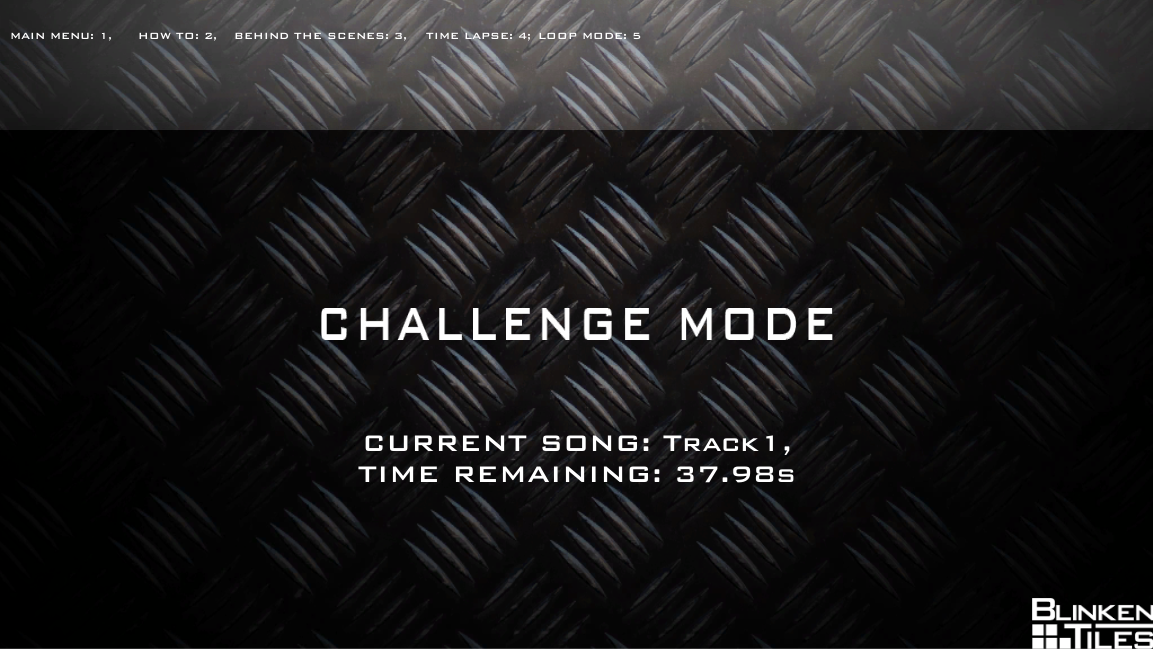
\includegraphics[width=0.88\textwidth]{images/PresScreen.png}
	\caption{Presentation-Screen im Challenge Mode}
	\label{fig:PresScreen}
\end{figure}

Die BlinkenTiles-Anwendung kommuniziert mit einem XML-File über das Internet mit dem Presentation-Programm. Die Hauptanwendung erstellt das File und legt es in einem Netzwerkordner ab. Dieser Teil wurde von Linda Schey implementiert. Die Presentation-Anwendung greift auf das File zu, parst die Textinformationen und speichert sie in entsprechenden Variablen. Abbildung \autoref{fig:XML} zeigt ein minimales Beispiel, welche Informationen so an den Presentation-Screen übermittelt werden können.

\begin{figure}[htbp]
	\centering
		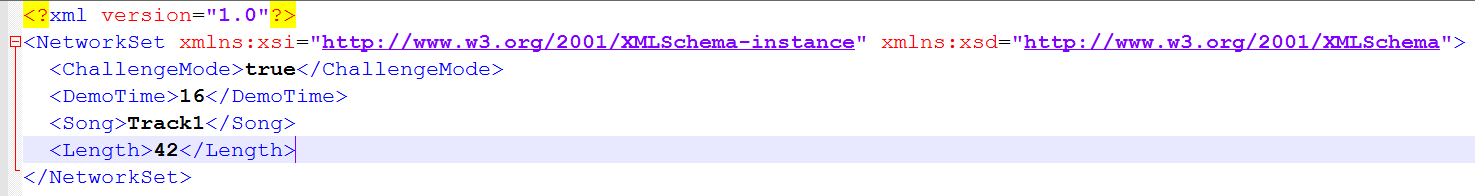
\includegraphics[width=1.0\textwidth]{images/XML.png}
	\caption{XML-File mit aktuellen Informationen für den Presentation-Screen }
	\label{fig:XML}
\end{figure}

Die Variablen werden dann an die einzelnen Codeelemente weitergegeben und für die Anzeigen verwendet. Der Countdown wird durch die übermittelte Länge des Liedes ermittelt und dann selbstständig dekrementiert. Endet der Challenge Mode, wird der Loop normal fortgesetzt.

\subsubsection{Spielfeld-Angaben}
Das Spielfeld, welches durch den Beamer auf den Boden projiziert wird, bietet ebenfalls eine gute Möglichkeit, direkt mit den Akteuren zu kommunizieren. Wenn der Challenge Mode startet, wird das Feld deswegen komplett weiß, eine Textinformation zeigt den Modus an und ein Countdown zählt die Beats zum Start herunter.\\
Eine Boolean-Variable checkt außerdem noch, ob sich gerade Personen auf dem Feld befinden. Wenn dies nicht der Fall ist, wird nach einer gewissen, konfigurierbaren Zeit der so genannte \textit{Idle Mode} gestartet. Um die Besucher zu motivieren, die Spielfläche zu betreten und um anzuzeigen, wie die Installation funktioniert, werden dabei Fußstapfen auf zufälligen Feldern verteilt. Nach einer gewissen Zeit ändern sie ihre Position. Die Fußstapfen sind Texturänderungen des Materials der Felder per Code. Ein mit einem Fußstapfen-Material belegtes Feld gilt als aktiv und wird so behandelt, als würde eine Person darauf stehen. Eine \emph{Update}-Methode überprüft regelmäßig, ob sich jemand auf das Spielfeld begibt. Ist dies der Fall, endet der Idle Mode sofort und die Fußstapfen verschwinden. Als kleine Auflockerung wurden nicht nur menschliche Fußstapfen verwendet, sondern auch die von Dinosauriern und Hunden (siehe Abbildung \autoref{fig:IdleAni}).

\begin{figure}[htbp]
	\centering
		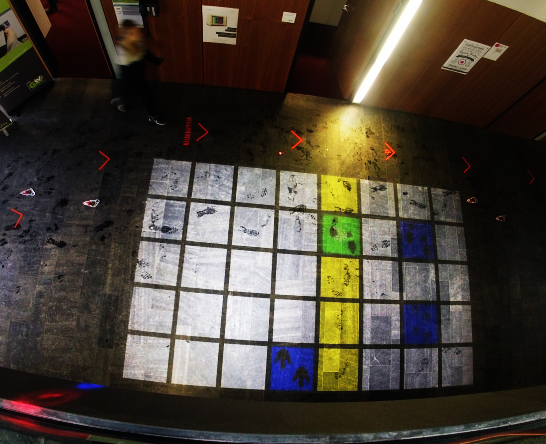
\includegraphics[width=0.9\textwidth]{images/IdleAni.png}
	\caption{Idle Modus mit Fußstapfen}
	\label{fig:IdleAni}
\end{figure}